\documentclass[border=10pt]{standalone}

\usepackage{tikz}
\usepackage{tikzsymbols}
\usetikzlibrary{calc,patterns,shapes.geometric}

\def\centerarc[#1](#2)(#3:#4:#5){\draw[#1] ($(#2)+({#5*cos(#3)},{#5*sin(#3)})$) arc (#3:#4:#5);}

\begin{document}
	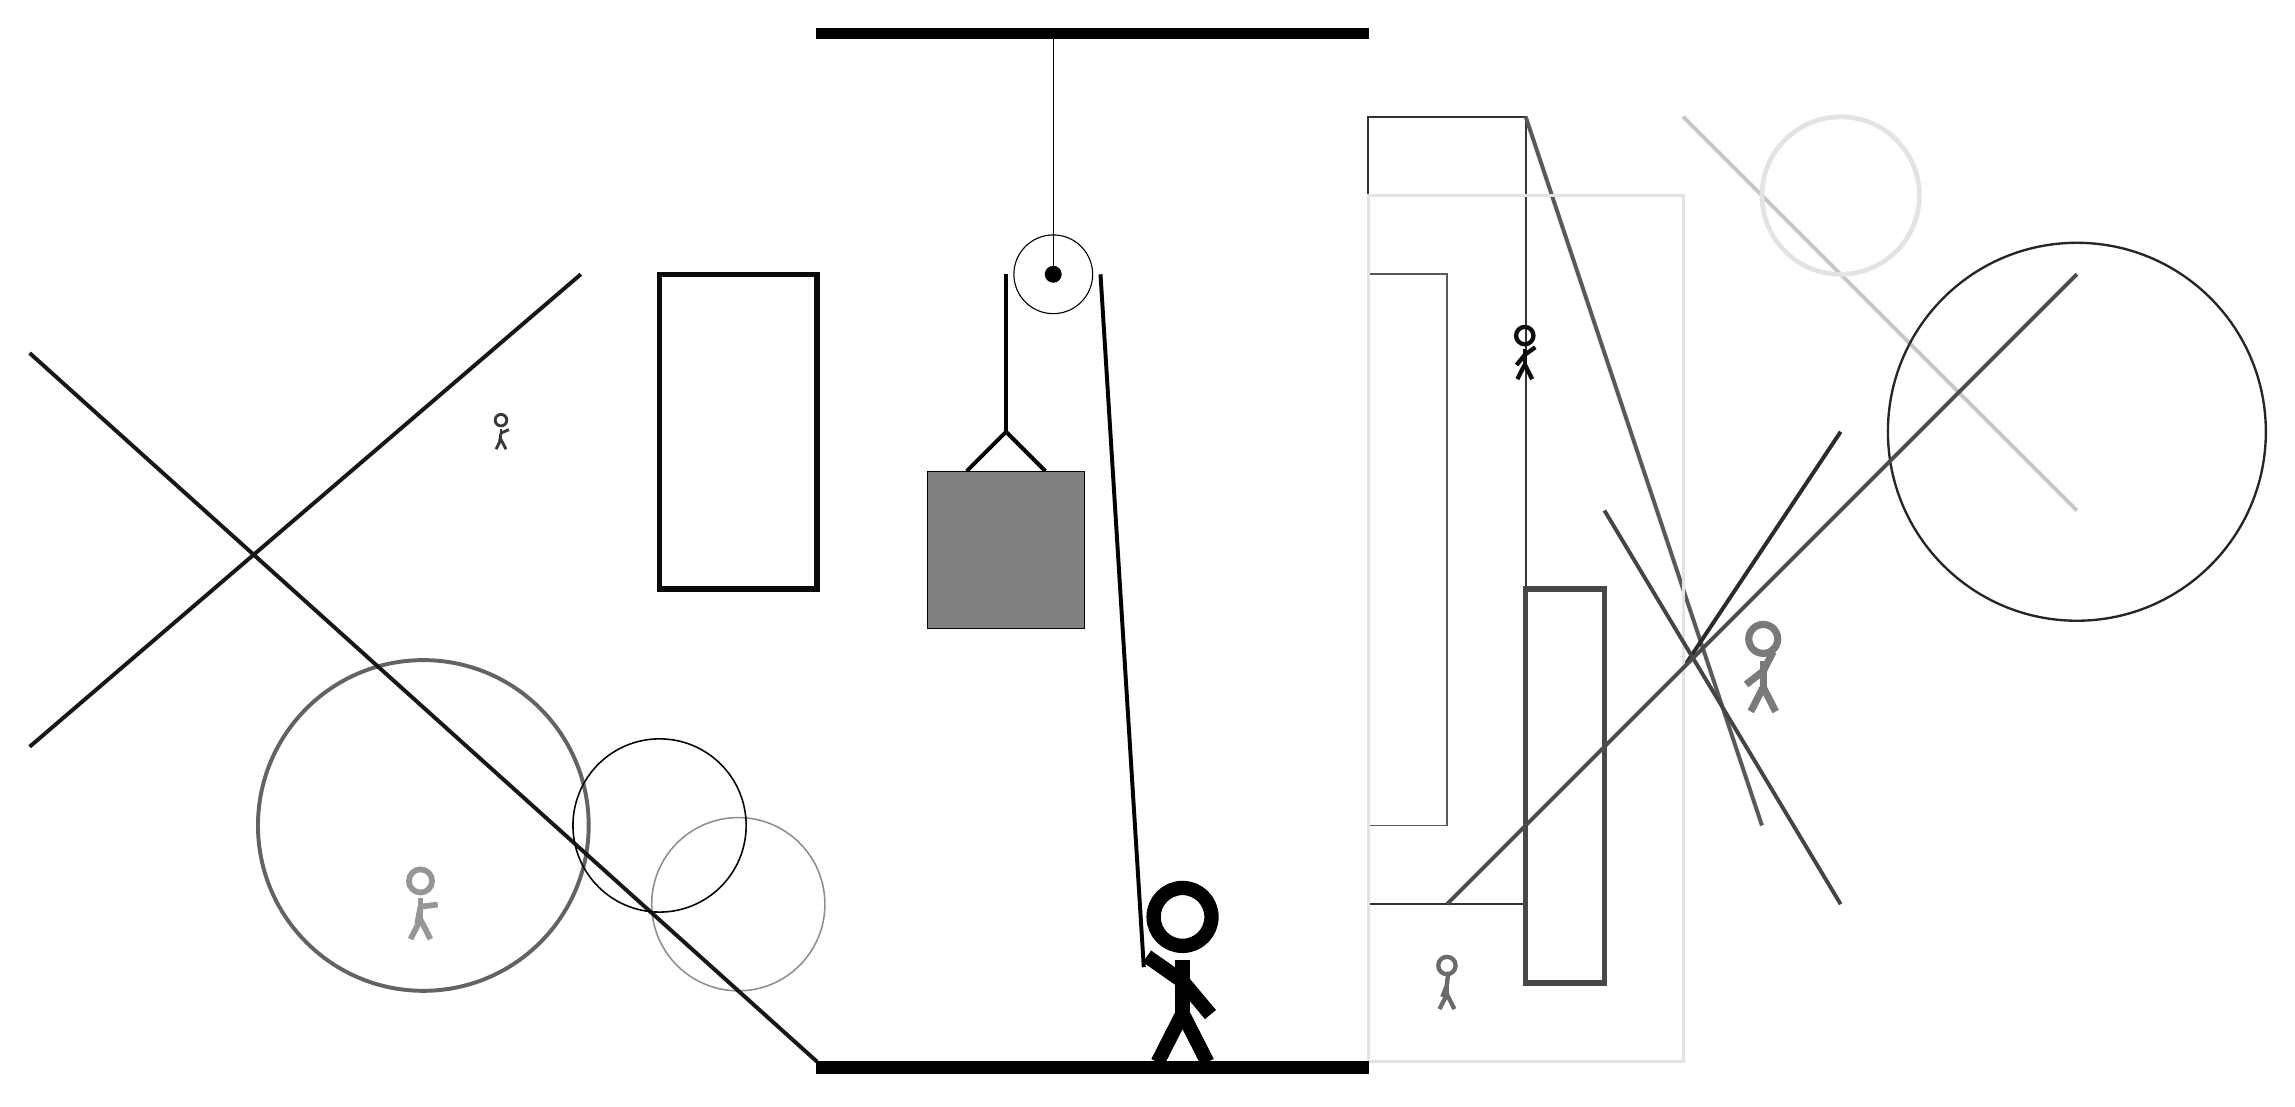
\begin{tikzpicture}
		%%%%% START %%%%%
		
		\draw[fill=black] (-2, 10) rectangle (5, 10.125);
		
		\draw (1, 7) circle (0.5);
		\draw[fill=black] (1, 7) circle (0.1);
		\draw (1, 10) -- (1, 7);
		
		\draw[line width=0.5mm] (-0.1, 4.5) -- (0.4, 5.0) -- (0.9, 4.5);
		\draw[fill=black!50] (-0.6, 4.5) rectangle (1.4, 2.5);
		
		\draw[line width=0.5mm] (0.4, 7) -- (0.4, 5.0);
		\centerarc[line width=0.5mm](1, 7)(0:180:0.6);
		\draw[line width=0.5mm](1.6, 7) -- (2.15, -1.8);
		
		\node at (2.6, -1.9) {\Strichmaxerl[10][-35][-50]};
		
		\node[line width=0.6mm, color=black!41] at (-7, -1) {\Strichmaxerl[4][79][7]};
		
		\draw[line width=0.5mm, color=black!22](9, 9) -- (14, 4);
		\draw[line width=0.3mm, color=black!80] (5, -1) rectangle (7, 9);
		\draw [line width=0.3mm, color=black!85](14, 5) circle (2.4);
		\draw[line width=0.5mm, color=black!91](-5, 7) -- (-12, 1);
		\draw [line width=0.6mm, color=black!11](11, 8) circle (1.0);
		\draw [line width=0.5mm, color=black!61](-7, 0) circle (2.1);
		
		\draw[line width=0.5mm, color=black!36] (7, 0) rectangle (7, 3);
		\draw[line width=0.7mm, color=black!96] (-4, 7) rectangle (-2, 3);
		\draw[line width=0.7mm, color=black!72] (7, -2) rectangle (8, 3);
		
		\draw [line width=0.2mm, color=black!44](-3, -1) circle (1.1);
		\node[line width=0.4mm, color=black!78] at (-6, 5) {\Strichmaxerl[2][81][23]};
		\node[line width=0.3mm, color=black!58] at (6, -2) {\Strichmaxerl[3][69][84]};
		
		\draw[line width=0.5mm, color=black!65](7, 9) -- (10, 0);
		\draw[line width=0.5mm, color=black!91](-2, -3) -- (-12, 6);
		\draw[line width=0.5mm, color=black!83](9, 2) -- (11, 5);
		\draw[line width=0.2mm, color=black!65] (6, 7) rectangle (5, 0);
		\draw [line width=0.2mm, color=black!98](-4, 0) circle (1.1);
		\draw[line width=0.4mm, color=black!11] (5, 8) rectangle (9, -3);
		\node[line width=0.5mm, color=black!95] at (7, 6) {\Strichmaxerl[3][51][36]};
		\node[line width=0.6mm, color=black!52] at (10, 2) {\Strichmaxerl[5][38][63]};
		
		\draw[line width=0.5mm, color=black!73](8, 4) -- (11, -1);
		
		\draw[line width=0.5mm, color=black!70](6, -1) -- (14, 7);
		
		\draw[fill=black] (-2, -3) rectangle (5, -3.15);
		
		%%%%% END %%%%%
	\end{tikzpicture}
\end{document}